\documentclass[12pt]{article}
\usepackage{setspace, graphicx, fullpage, amssymb, amsmath, epsfig, natbib, array, multirow, hyperref}
\usepackage{amsfonts, bm} 
\usepackage{dcolumn}
\usepackage{subfigure, float} 
\usepackage[margin=1in]{geometry} 
\usepackage{verbatim}
\usepackage{url}
\usepackage{enumerate}
\usepackage{morefloats}
\newcolumntype{d}[1]{D{.}{.}{#1}} 



\begin{document}
	
\begin{center}
	\Large 05 April 2017
\end{center}

\section{Overview}

Items for which further work was previously requested by one or both of you were as follows:
\begin{itemize}
	\item Develop a formal model for the impact of reelection on party calls
	
	\item Estimate the House models with two party vote share instead of overall vote share
	
	\item Summarize readings relevant to this paper
	
	\item Continue to rework the paper
\end{itemize}
William has gone through the process of developing the formal model with me. 

Additionally, during this time we discussed the differences between the vote percent variable that we have been using in the House (overall vote percent of candidate) and the Senate (two party vote share). We did not believe that this would cause meaningful differences, but recognize that this is something we want to deal with in some way before sending the paper out for review. Thankfully, the presidential vote share data for Congressional districts also contained this measure, so I have included a section which shows the results when this measure is instead used. I include the tables with these measures in this section in order to provide comparability.

In the section following that, I provide what I consider to be a one sentence summary of the relevant parts of things we are referencing or might reference, with other important points included below this.

Finally, I have made some adjustments to the article draft in the final section.



\section{House Tables and Figures with 2 Party Vote Share}

As expected moving to two party vote share (rather than total vote share) provides little substantive difference to the results. This also includes a change to how unopposed candidates are scaled. Since Jacobson's data have unopposed candidates vote share as an NA value, rather than set to 100\% as in the LEP data, I took William's advice and subtracted the mean from this variable and set it to 0. I include a coefficient plot with the unopposed missing values instead set to 100 without centering the data on 0 to show that this produces essentially no difference. Ultimately our results are robust to these changes and we should simply go with one specification and note that it doesn't matter in the paper or an appendix.

\begin{table}
	\begin{center}
		\caption{Regressions with 2 Party Vote Share}
		\begin{tabular}{l c c c c }
			\hline
			& Democrats & Republicans & Majority & Minority \\
			\hline
			ideological\_extremism & $8.361^{***}$  & $5.680^{***}$  & $6.680^{***}$  & $8.436^{***}$  \\
			& $(0.168)$      & $(0.205)$      & $(0.156)$      & $(0.202)$      \\
			pfrate100              & $0.641^{***}$  & $0.407^{***}$  & $0.541^{***}$  & $0.601^{***}$  \\
			& $(0.015)$      & $(0.019)$      & $(0.015)$      & $(0.019)$      \\
			vote\_share            & $-0.051^{***}$ & $0.046^{*}$    & $-0.118^{***}$ & $-0.094^{***}$ \\
			& $(0.013)$      & $(0.021)$      & $(0.014)$      & $(0.019)$      \\
			pres\_vote\_share      & $0.094^{***}$  & $-0.111^{***}$ & $0.198^{***}$  & $0.180^{***}$  \\
			& $(0.011)$      & $(0.019)$      & $(0.012)$      & $(0.018)$      \\
			south                  & $-2.669^{***}$ & $3.624^{***}$  & $-2.216^{***}$ & $-0.746^{*}$   \\
			& $(0.273)$      & $(0.325)$      & $(0.242)$      & $(0.312)$      \\
			female                 & $0.707^{*}$    & $-0.196$       & $0.124$        & $2.161^{***}$  \\
			& $(0.349)$      & $(0.570)$      & $(0.399)$      & $(0.443)$      \\
			afam                   & $-0.290$       & $5.143$        & $-2.717^{***}$ & $3.357^{***}$  \\
			& $(0.437)$      & $(2.993)$      & $(0.531)$      & $(0.605)$      \\
			latino                 & $1.807^{***}$  & $2.169$        & $2.235^{***}$  & $3.360^{***}$  \\
			& $(0.507)$      & $(1.152)$      & $(0.618)$      & $(0.705)$      \\
			seniority              & $0.055$        & $-0.347^{***}$ & $0.022$        & $-0.006$       \\
			& $(0.031)$      & $(0.050)$      & $(0.034)$      & $(0.041)$      \\
			freshman               & $0.035$        & $0.952^{*}$    & $0.285$        & $-0.457$       \\
			& $(0.348)$      & $(0.458)$      & $(0.344)$      & $(0.440)$      \\
			bestgrosswart          & $-0.036^{*}$   & $-0.254^{***}$ & $-0.173^{***}$ & $-0.175^{***}$ \\
			& $(0.018)$      & $(0.025)$      & $(0.018)$      & $(0.022)$      \\
			leader                 & $1.940^{**}$   & $2.771^{***}$  & $2.424^{***}$  & $1.893^{**}$   \\
			& $(0.596)$      & $(0.763)$      & $(0.641)$      & $(0.664)$      \\
			power                  & $1.865^{***}$  & $2.799^{***}$  & $2.977^{***}$  & $1.229^{***}$  \\
			& $(0.275)$      & $(0.372)$      & $(0.268)$      & $(0.363)$      \\
			chair                  & $2.461^{***}$  & $9.423^{***}$  & $1.886^{***}$  & $-7.738$       \\
			& $(0.499)$      & $(0.792)$      & $(0.444)$      & $(4.721)$      \\
			(Intercept)            & $20.938^{***}$ & $55.310^{***}$ & $28.554^{***}$ & $15.808^{***}$ \\
			& $(1.478)$      & $(2.139)$      & $(1.380)$      & $(2.087)$      \\
			\hline
			R$^2$                  & 0.631          & 0.292          & 0.564          & 0.461          \\
			Adj. R$^2$             & 0.630          & 0.290          & 0.562          & 0.459          \\
			Num. obs.              & 4879           & 3906           & 5045           & 3740           \\
			RMSE                   & 7.430          & 8.931          & 7.633          & 8.158          \\
			\hline
			\multicolumn{5}{l}{\scriptsize{$^{***}p<0.001$, $^{**}p<0.01$, $^*p<0.05$}}
		\end{tabular}
	\end{center}
\end{table}

\begin{table}
	\begin{center}
		\caption{Regressions with Vote Percent}
		\begin{tabular}{l c c c c }
			\hline
			& Democrats & Republicans & Majority & Minority \\
			\hline
			ideological\_extremism & $8.320^{***}$  & $5.781^{***}$  & $6.581^{***}$  & $8.655^{***}$  \\
			& $(0.169)$      & $(0.207)$      & $(0.157)$      & $(0.201)$      \\
			pfrate100              & $0.636^{***}$  & $0.423^{***}$  & $0.524^{***}$  & $0.637^{***}$  \\
			& $(0.016)$      & $(0.020)$      & $(0.015)$      & $(0.020)$      \\
			votepct                & $-0.036^{***}$ & $-0.001$       & $-0.087^{***}$ & $-0.066^{***}$ \\
			& $(0.009)$      & $(0.014)$      & $(0.009)$      & $(0.013)$      \\
			pres\_vote\_share      & $0.093^{***}$  & $-0.098^{***}$ & $0.195^{***}$  & $0.165^{***}$  \\
			& $(0.011)$      & $(0.019)$      & $(0.011)$      & $(0.017)$      \\
			south                  & $-2.418^{***}$ & $3.616^{***}$  & $-1.680^{***}$ & $-0.395$       \\
			& $(0.281)$      & $(0.337)$      & $(0.251)$      & $(0.316)$      \\
			female                 & $0.536$        & $-0.185$       & $-0.159$       & $2.090^{***}$  \\
			& $(0.355)$      & $(0.575)$      & $(0.405)$      & $(0.443)$      \\
			afam                   & $-0.530$       & $4.968$        & $-2.968^{***}$ & $3.253^{***}$  \\
			& $(0.442)$      & $(2.981)$      & $(0.536)$      & $(0.609)$      \\
			latino                 & $1.732^{***}$  & $2.309^{*}$    & $2.803^{***}$  & $2.995^{***}$  \\
			& $(0.516)$      & $(1.157)$      & $(0.628)$      & $(0.706)$      \\
			seniority              & $0.049$        & $-0.337^{***}$ & $0.014$        & $0.003$        \\
			& $(0.031)$      & $(0.050)$      & $(0.034)$      & $(0.041)$      \\
			freshman               & $-0.043$       & $0.945^{*}$    & $0.220$        & $-0.310$       \\
			& $(0.358)$      & $(0.463)$      & $(0.349)$      & $(0.446)$      \\
			bestgrosswart          & $-0.036$       & $-0.258^{***}$ & $-0.181^{***}$ & $-0.166^{***}$ \\
			& $(0.019)$      & $(0.025)$      & $(0.019)$      & $(0.023)$      \\
			leader                 & $1.968^{**}$   & $2.756^{***}$  & $2.586^{***}$  & $1.788^{**}$   \\
			& $(0.601)$      & $(0.763)$      & $(0.649)$      & $(0.655)$      \\
			power                  & $1.805^{***}$  & $2.943^{***}$  & $3.012^{***}$  & $1.086^{**}$   \\
			& $(0.276)$      & $(0.375)$      & $(0.269)$      & $(0.362)$      \\
			chair                  & $2.469^{***}$  & $9.494^{***}$  & $1.823^{***}$  & $-7.964$       \\
			& $(0.499)$      & $(0.799)$      & $(0.445)$      & $(4.656)$      \\
			(Intercept)            & $24.013^{***}$ & $53.078^{***}$ & $36.309^{***}$ & $17.696^{***}$ \\
			& $(1.581)$      & $(2.211)$      & $(1.496)$      & $(2.057)$      \\
			\hline
			R$^2$                  & 0.629          & 0.300          & 0.563          & 0.474          \\
			Adj. R$^2$             & 0.628          & 0.298          & 0.562          & 0.472          \\
			Num. obs.              & 4740           & 3804           & 4902           & 3642           \\
			RMSE                   & 7.385          & 8.891          & 7.575          & 8.045          \\
			\hline
			\multicolumn{5}{l}{\scriptsize{$^{***}p<0.001$, $^{**}p<0.01$, $^*p<0.05$}}
		\end{tabular}
	\end{center}
\end{table}

\begin{table}
	\begin{center}
		\caption{Table 3 Replication with 2 Party Vote Share}
		\begin{tabular}{l c c c c c c }
			\hline
			& \multicolumn{3}{c}{Democrats} & \multicolumn{3}{c}{Republicans} \\
			\cline{2-7}
			& 97th & 102nd & 107th & 97th & 102nd & 107th \\
			\hline
			ideological\_extremism & $9.23^{***}$  & $4.97^{***}$ & $0.03$        & $5.29^{***}$ & $5.31^{***}$  & $0.26$        \\
			& $(0.55)$      & $(0.67)$     & $(1.44)$      & $(0.69)$     & $(0.82)$      & $(0.60)$      \\
			pfrate100              & $1.04^{***}$  & $0.72^{***}$ & $0.76^{*}$    & $0.55^{***}$ & $0.49^{***}$  & $0.45^{***}$  \\
			& $(0.07)$      & $(0.08)$     & $(0.35)$      & $(0.07)$     & $(0.09)$      & $(0.10)$      \\
			pres\_vote\_share      & $0.14^{**}$   & $0.19^{***}$ & $0.35^{***}$  & $0.20^{**}$  & $0.27^{**}$   & $0.18^{***}$  \\
			& $(0.05)$      & $(0.05)$     & $(0.06)$      & $(0.06)$     & $(0.09)$      & $(0.04)$      \\
			south                  & $-5.09^{***}$ & $-1.28$      & $-2.85^{*}$   & $1.63$       & $0.01$        & $1.67^{**}$   \\
			& $(1.03)$      & $(0.77)$     & $(1.17)$      & $(1.13)$     & $(1.26)$      & $(0.50)$      \\
			vote\_share            & $-0.11^{*}$   & $-0.13^{**}$ & $-0.25^{***}$ & $0.03$       & $-0.12$       & $-0.07$       \\
			& $(0.05)$      & $(0.04)$     & $(0.07)$      & $(0.06)$     & $(0.07)$      & $(0.04)$      \\
			female                 & $3.23$        & $-1.61$      & $2.11$        & $-4.05^{*}$  & $-2.96$       & $-1.47$       \\
			& $(1.83)$      & $(1.20)$     & $(1.15)$      & $(1.99)$     & $(2.50)$      & $(0.85)$      \\
			afam                   & $-0.77$       & $-1.82$      & $-1.91$       &              & $1.34$        & $-2.68$       \\
			& $(2.10)$      & $(1.54)$     & $(1.66)$      &              & $(6.82)$      & $(3.65)$      \\
			latino                 & $4.34$        & $1.98$       & $1.04$        & $-2.16$      & $2.71$        & $0.45$        \\
			& $(2.68)$      & $(1.76)$     & $(1.83)$      & $(5.73)$     & $(7.06)$      & $(1.53)$      \\
			seniority              & $0.18$        & $0.08$       & $-0.04$       & $-0.05$      & $-0.84^{***}$ & $-0.12$       \\
			& $(0.12)$      & $(0.10)$     & $(0.13)$      & $(0.17)$     & $(0.16)$      & $(0.08)$      \\
			freshman               & $0.50$        & $-0.04$      & $1.30$        & $2.65^{*}$   & $3.40$        & $0.66$        \\
			& $(1.31)$      & $(1.14)$     & $(1.74)$      & $(1.31)$     & $(1.94)$      & $(0.78)$      \\
			bestgrosswart          & $0.02$        & $-0.09$      & $0.19^{*}$    & $0.02$       & $0.04$        & $0.09$        \\
			& $(0.08)$      & $(0.08)$     & $(0.09)$      & $(0.09)$     & $(0.11)$      & $(0.05)$      \\
			leader                 & $5.86^{*}$    & $2.22$       & $0.59$        & $0.24$       & $3.70$        & $2.98^{*}$    \\
			& $(2.68)$      & $(1.92)$     & $(2.33)$      & $(2.40)$     & $(2.47)$      & $(1.26)$      \\
			power                  & $1.89$        & $1.49$       & $-0.61$       & $-0.60$      & $-0.17$       & $0.20$        \\
			& $(1.03)$      & $(0.88)$     & $(1.25)$      & $(1.29)$     & $(1.52)$      & $(0.62)$      \\
			chair                  & $2.29$        & $1.16$       & $2.76$        &              & $-2.39$       & $1.12$        \\
			& $(1.58)$      & $(1.32)$     & $(6.35)$      &              & $(6.72)$      & $(0.90)$      \\
			(Intercept)            & $-22.89^{**}$ & $17.18^{*}$  & $-9.64$       & $13.47$      & $21.64^{*}$   & $37.92^{***}$ \\
			& $(7.04)$      & $(7.32)$     & $(34.45)$     & $(8.03)$     & $(8.57)$      & $(10.18)$     \\
			\hline
			R$^2$                  & 0.80          & 0.68         & 0.39          & 0.53         & 0.55          & 0.50          \\
			Adj. R$^2$             & 0.79          & 0.66         & 0.35          & 0.50         & 0.51          & 0.47          \\
			Num. obs.              & 245           & 267          & 214           & 193          & 172           & 228           \\
			RMSE                   & 5.74          & 4.87         & 6.21          & 5.58         & 6.53          & 3.35          \\
			\hline
			\multicolumn{7}{l}{\scriptsize{$^{***}p<0.001$, $^{**}p<0.01$, $^*p<0.05$}}
		\end{tabular}
	\end{center}
\end{table}

\begin{table}
	\begin{center}
		\caption{Table 3 Replications with Vote Percent}
		\begin{tabular}{l c c c c c c }
			\hline
			& \multicolumn{3}{c}{Democrats} & \multicolumn{3}{c}{Republicans} \\
			\cline{2-7}
			& 97th & 102nd & 107th & 97th & 102nd & 107th \\
			\hline
			ideological\_extremism & $9.39^{***}$  & $5.13^{***}$ & $0.14$       & $5.28^{***}$ & $6.25^{***}$  & $0.25$        \\
			& $(0.54)$      & $(0.69)$     & $(1.55)$     & $(0.70)$     & $(0.79)$      & $(0.61)$      \\
			pfrate100              & $1.03^{***}$  & $0.69^{***}$ & $0.79^{*}$   & $0.51^{***}$ & $0.52^{***}$  & $0.43^{***}$  \\
			& $(0.07)$      & $(0.08)$     & $(0.38)$     & $(0.08)$     & $(0.09)$      & $(0.11)$      \\
			pres\_vote\_share      & $0.15^{**}$   & $0.14^{**}$  & $0.23^{***}$ & $0.22^{**}$  & $0.22^{*}$    & $0.16^{***}$  \\
			& $(0.05)$      & $(0.05)$     & $(0.06)$     & $(0.07)$     & $(0.09)$      & $(0.04)$      \\
			south                  & $-4.00^{***}$ & $-1.29$      & $-2.97^{*}$  & $1.46$       & $0.05$        & $1.69^{**}$   \\
			& $(1.02)$      & $(0.80)$     & $(1.26)$     & $(1.18)$     & $(1.29)$      & $(0.53)$      \\
			votepct                & $-0.08^{*}$   & $-0.03$      & $-0.04$      & $0.06$       & $-0.01$       & $-0.02$       \\
			& $(0.03)$      & $(0.03)$     & $(0.05)$     & $(0.05)$     & $(0.04)$      & $(0.02)$      \\
			female                 & $0.09$        & $-1.70$      & $2.51^{*}$   & $-4.16^{*}$  & $-2.40$       & $-1.40$       \\
			& $(2.09)$      & $(1.22)$     & $(1.19)$     & $(1.99)$     & $(2.37)$      & $(0.86)$      \\
			afam                   & $-2.61$       & $-2.03$      & $-1.58$      &              & $3.22$        & $-2.88$       \\
			& $(2.14)$      & $(1.58)$     & $(1.70)$     &              & $(6.48)$      & $(3.66)$      \\
			latino                 & $4.24$        & $2.67$       & $0.50$       & $-1.37$      & $3.65$        & $0.74$        \\
			& $(2.94)$      & $(1.90)$     & $(1.86)$     & $(5.70)$     & $(6.70)$      & $(1.54)$      \\
			seniority              & $0.09$        & $0.07$       & $-0.14$      & $-0.05$      & $-0.73^{***}$ & $-0.17^{*}$   \\
			& $(0.12)$      & $(0.10)$     & $(0.13)$     & $(0.17)$     & $(0.16)$      & $(0.08)$      \\
			freshman               & $-1.06$       & $0.18$       & $-0.01$      & $3.14^{*}$   & $4.32^{*}$    & $0.48$        \\
			& $(1.45)$      & $(1.20)$     & $(1.99)$     & $(1.34)$     & $(1.86)$      & $(0.80)$      \\
			bestgrosswart          & $0.13$        & $-0.08$      & $0.28^{**}$  & $0.06$       & $0.04$        & $0.13^{*}$    \\
			& $(0.08)$      & $(0.08)$     & $(0.10)$     & $(0.09)$     & $(0.12)$      & $(0.05)$      \\
			leader                 & $7.15^{*}$    & $1.98$       & $0.85$       & $0.26$       & $3.81$        & $3.00^{*}$    \\
			& $(2.90)$      & $(1.95)$     & $(2.38)$     & $(2.40)$     & $(2.36)$      & $(1.26)$      \\
			power                  & $0.95$        & $1.50$       & $-1.30$      & $-1.11$      & $0.42$        & $0.04$        \\
			& $(1.03)$      & $(0.90)$     & $(1.30)$     & $(1.34)$     & $(1.49)$      & $(0.64)$      \\
			chair                  & $2.66$        & $1.24$       & $4.38$       &              & $-0.96$       & $1.27$        \\
			& $(1.53)$      & $(1.35)$     & $(6.43)$     &              & $(6.36)$      & $(0.93)$      \\
			(Intercept)            & $-18.53^{**}$ & $23.84^{**}$ & $-3.50$      & $11.65$      & $20.72^{*}$   & $41.67^{***}$ \\
			& $(6.78)$      & $(7.38)$     & $(36.62)$    & $(8.00)$     & $(8.96)$      & $(10.37)$     \\
			\hline
			R$^2$                  & 0.81          & 0.66         & 0.37         & 0.54         & 0.58          & 0.50          \\
			Adj. R$^2$             & 0.80          & 0.64         & 0.32         & 0.51         & 0.54          & 0.47          \\
			Num. obs.              & 234           & 262          & 208          & 186          & 163           & 218           \\
			RMSE                   & 5.53          & 4.96         & 6.30         & 5.57         & 6.18          & 3.35          \\
			\hline
			\multicolumn{7}{l}{\scriptsize{$^{***}p<0.001$, $^{**}p<0.01$, $^*p<0.05$}}
		\end{tabular}
	\end{center}
\end{table}

\begin{figure}[H]
	\centering
	\caption{Figure 2 Replication, 2 Party Vote Share, Centered at 0}
	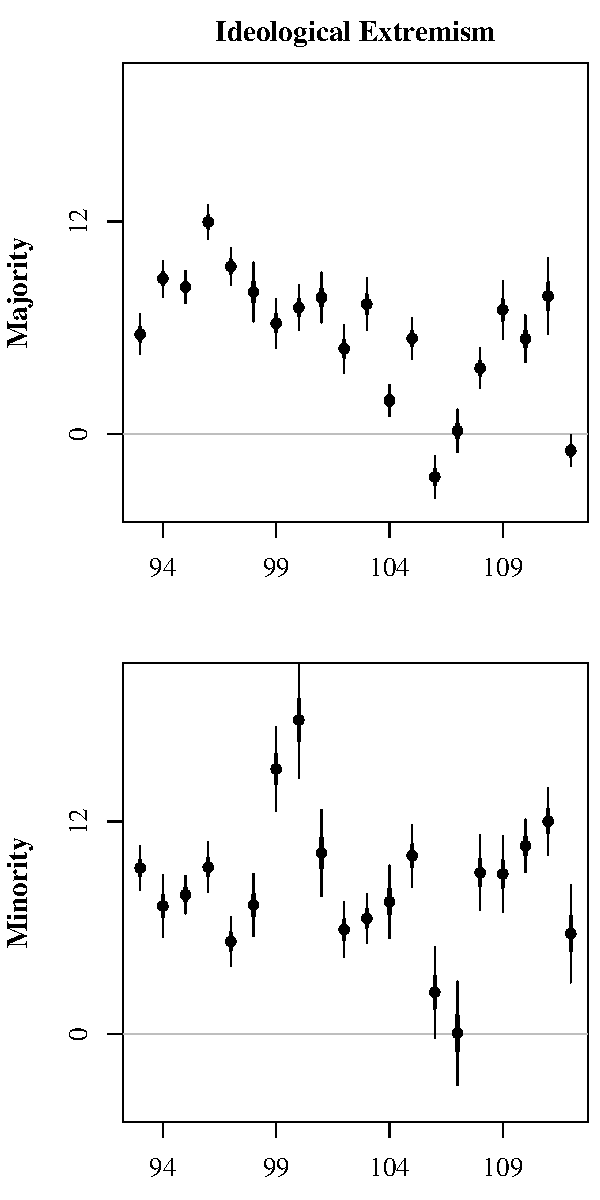
\includegraphics[width = 10cm]{C:/Users/Ethan/Documents/GitHub/partycalls/plots/who-heeds-figure2-replication_vote_share.pdf}
\end{figure}

\begin{figure}[H]
	\centering
	\caption{Figure 2 Replication, 2 Party Vote Share, Unopposed Candidates set to 100\%}
	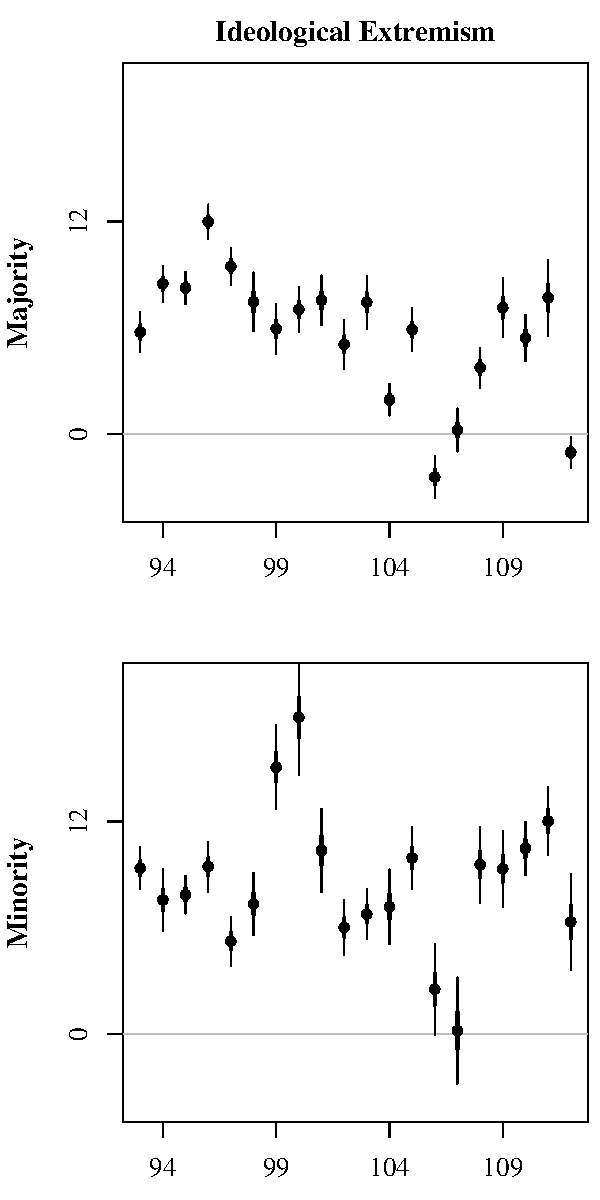
\includegraphics[width = 10cm]{C:/Users/Ethan/Documents/GitHub/partycalls/plots/who-heeds-figure2-replication_vote_share_b.pdf}
\end{figure}

\begin{figure}[H]
	\centering
	\caption{Figure 2 Replication, Vote Percent}
	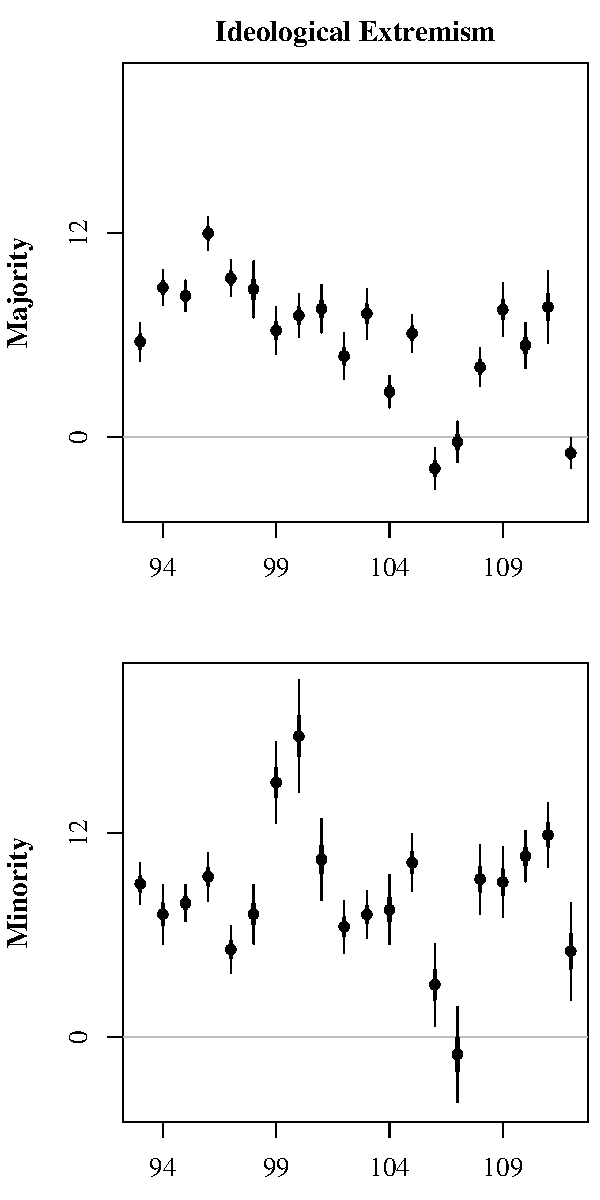
\includegraphics[width = 10cm]{C:/Users/Ethan/Documents/GitHub/partycalls/plots/who-heeds-figure2-replication_lm.pdf}
\end{figure}



\pagebreak



\section{Summary of Related Books and Articles}

\noindent
\textbf{Levitt (1996), ``How Do Senators Vote?''}

In election years, Senators' pay more heed to the desires of their state than in the rest of their term.

The methodology of the reelection section is as follows:
\begin{itemize}
	\item Divides by years, rather than Congresses
	
	\item Uses ADA scores of various groups of MCs (both in the House and Senate) as proxies for state, constituency, party
	
	\item Uses differences between same-state Senators to get ideology measure (rather than estimate by roll calls or use measures that do)
	
	\item The above values are regressed with coefficients constrained to add up to 1 and reported in tables, these are referred to as weights in the utility function
	
	\item The weights from an election year are compared with those of Senators 4 or more years from reelection (since the method of comparison is unspecified, I assume it to be a simple comparison such as a paired $z$-test)
\end{itemize}

\noindent
\textbf{Lee (2009) \textit{Beyond Ideology}}

Much of what happens in Congress that is attributed to ideological conflict is actually the result of partisan conflict.

\begin{itemize}	
	\item It is necessary to disentangle party and ideology
	
	\item Party brand held to be important to members (no discussion of variation among members)
	
	\item Issues are selected in order to put parties in conflict, which is seen as boosting the party brand
	
	\item Roll call votes can be a tool for embarrassing the opposition by making them go on record for or against controversial issues
	
	\item Greater time between elections in Senate decreases focus on electoral stakes
	
	\item Actions taken to benefit the party brand held to be net benefit for members
\end{itemize}

\noindent
\textbf{Carson et al. (2010) ``The Electoral Costs of Party Loyalty in Congress''}

Voters punish members who are perceived to merely vote the party line.

\noindent
\textbf{Canes-Wrone, Brady \& Cogan (2002) ``Out of Step, Out of Office''}

Members who take positions on issues which differ from those of their district are punished by voters.

\noindent
\textbf{Theriault (2013) \textit{The Gingrich Senators}}

Senators who came from House service with Newt Gingrich brought norms of intense partisan conflict which reshaped the Senate, leading it into a new hyper partisan era.

\begin{itemize}
	\item Divides post-WWII Senate into 3 eras: Textbook Senate, Individualized Senate, Partisan Senate
		
	\item Southern Democrats and Gingrich Senators have each acted as sub-parties at different times; the former brought about compromise, the latter conflict
\end{itemize}

\noindent
\textbf{Smith (2014) \textit{The Senate Syndrome}}

The Senate has in recent decades become gridlocked as the result of increased media attention, party polarization, and trends resulting from past rule changes. 



\pagebreak



\section{Paper, Draft 3}

\subsection{Introduction}

Minozzi \& Volden (2013) demonstrated that party unity on legislation comes less often from the pressuring of moderates but instead from calling on members to coalesce out of shared interest. Members of all ideological stripes will have reasons to vote out of step with the party. However, the responsive extremists hypothesis developed by Minozzi \& Volden held that when the party called on its members that it was those extreme members who would get in line. This was tested by sorting roll call votes into party influenced votes and party free votes and estimating the impact of member ideology on decision to respond to party influence.

This paper is written as an attempt to replicate this finding, extending the units of analysis to include the Senate and the period of analysis to Congresses 93-112. This allows us to test the responsive extremists hypothesis in both chambers, considering also times which both chambers are held to have become more extreme. The Senate allows not only for the extension of the results, but also for consideration of how proximity to election influences members' response to the party.

Following Mayhew (1974) we assume reelection to be chief among the goals of members of Congress. Levitt (1996) finds that proximity to reelection induces Senators to more strongly take their constituents' preferences into account. Canes-Wrone, Brady \& Cogan (2002) shows that members who stray to far from the preferences of their district are less likely to be reelected. While this would initially seem to imply that members would act according to the preferences of their district above those of their party, we know from Lee (2009) that the name brands of parties confer advantages to members in ways which offset the costs of party unity. Carson, Koger, Lebo \& Young (2010) find, however, that voters are likely to punish members they perceive to lack principles beyond party unity. 

We hypothesize that members approaching reelection will take strategic votes against the party to differentiate themselves. We expect this to be present primarily in votes when the party is calling, since it provides the strongest signal to constituents that a member is taking their desires into account. Still, given that the responsive extremists hypothesis was originally tested in the House (in which members are always up for reelection at the end of a Congress) we expect the effect to not be so strong as to overwhelm members' responsiveness to the party.

\subsection{Replication with Extension}

In this section we show that the results from Minozzi \& Volden (2013) hold when analysis is extended into later Congresses and the Senate. We draw on Congressional roll call data for Congresses 93-112 to measure member behavior. We replicate their iterative roll call sorting algorithm to obtain party influenced and party free votes. The set of party free votes from one iteration is used as the votes for calculating party free ideology in the next, with ideological extremism being this measure with sign reversed for Democrats.\footnote{A more thorough overview of the methodology is detailed in an appendix.}

We find that in both chambers and both parties, baseline party unity is most present near the party median, with a dropoff as one approaches either tail. However, party call votes demonstrate only a dropoff as one approaches the less extreme end of the party. This is shown in figures with $y$ axes denoting the percentage of votes cast in line with a majority of the party and $x$ axes member ideological extremism.

\begin{figure}[H]
	\centering
	\caption{House Rate of Voting With Party by Vote Type}
	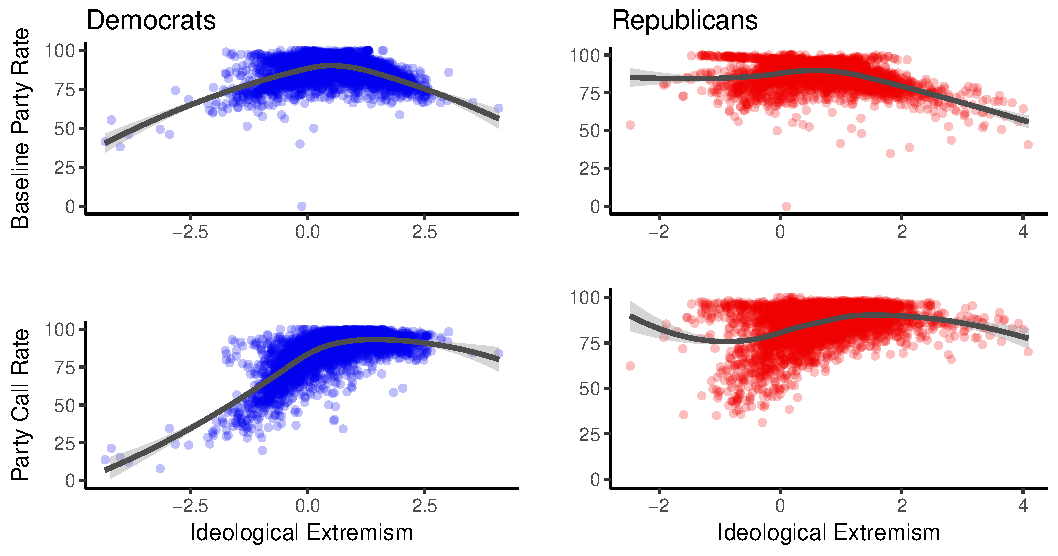
\includegraphics[width = \textwidth]{C:/Users/Ethan/Documents/GitHub/partycalls/plots/house_responsiveness_plot.pdf}
\end{figure}

\begin{figure}[H]
	\centering
	\caption{Senate Rate of Voting With Party by Vote Type}
	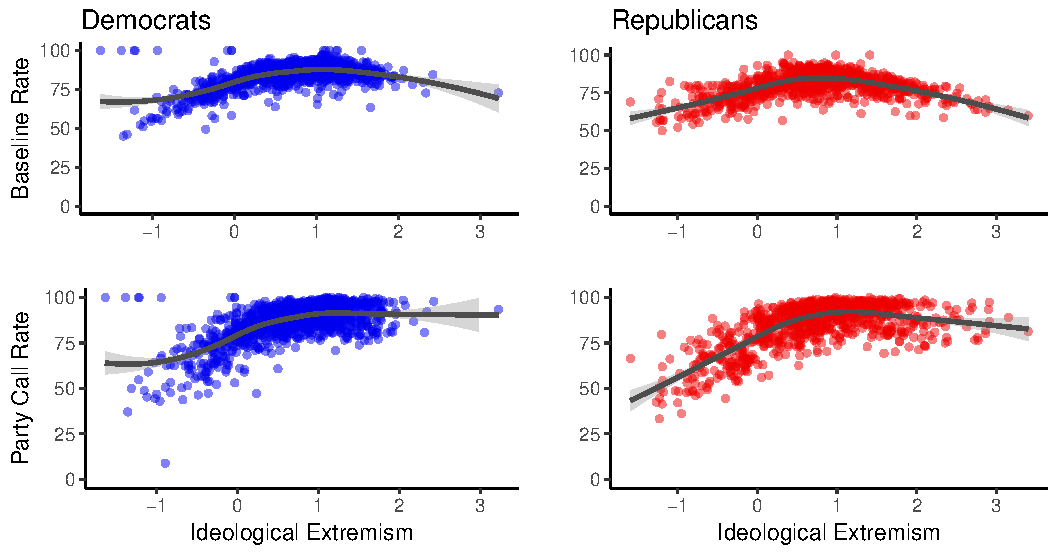
\includegraphics[width = \textwidth]{C:/Users/Ethan/Documents/GitHub/partycalls/plots/senate_responsiveness_plot.pdf}
\end{figure}

We also note that the number of party call votes in both chambers of Congress during the period of analysis are on an upward trend. We believe this trend merits further investigation, but initially take it to echo arguments such as those of Lee (2009), Theriault (2013), and Smith (2014) that Congressional parties have become increasingly divided by party and ideology. 

\begin{figure}[H]
	\centering
	\caption{Party Calls as a Percentage of Votes, Congresses 93-112}
	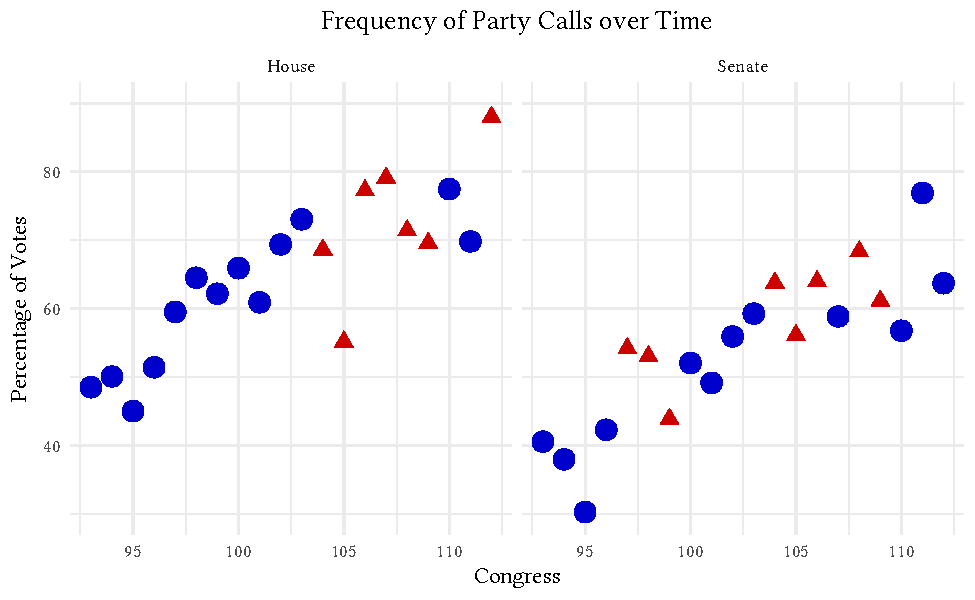
\includegraphics[width = \textwidth]{C:/Users/Ethan/Documents/GitHub/partycalls/plots/party_call_percent_both.pdf}
\end{figure}

Pooled regressions with members divided by party and majority status broadly show the responsive extremists hypothesis to hold in the extended set of cases we consider. Though they differ in strength between parties, ideological extremism and rate of voting with majority of non party call votes both carry substantive predictive power in determining responsiveness by to party calls. 

In both chambers we find that southern Democrats are less responsive to the party than are other Democrats. We also note that the power committee variable we constructed for the Senate (based on membership in a top 4 committee) carries little predictive power, either in terms of substantive power or statistical significance. This is not entirely unexpected, since this is a variable we included less because we believed it had meaning to Senators and more for model comparability. We also note that in both chambers increased same party presidential vote share within one's constituency makes Democrats more likely to respond to a party call but reduces the chances of a Republican doing so.

\begin{table}[H]
	\begin{center}
		\caption{House Responsiveness to Party Calls, Pooled Regressions}
		%\footnotesize
		\begin{tabular}{l c c c c }
			\hline
			& Democrats & Republicans & Majority & Minority \\
			\hline
			ideological\_extremism & $8.34^{***}$  & $5.84^{***}$  & $6.65^{***}$  & $8.73^{***}$  \\
			& $(0.17)$      & $(0.21)$      & $(0.16)$      & $(0.20)$      \\
			pfrate100              & $0.64^{***}$  & $0.41^{***}$  & $0.52^{***}$  & $0.64^{***}$  \\
			& $(0.02)$      & $(0.02)$      & $(0.01)$      & $(0.02)$      \\
			votepct                & $-0.04^{***}$ & $-0.00$       & $-0.09^{***}$ & $-0.07^{***}$ \\
			& $(0.01)$      & $(0.01)$      & $(0.01)$      & $(0.01)$      \\
			pres\_votepct          & $0.09^{***}$  & $-0.09^{***}$ & $0.20^{***}$  & $0.16^{***}$  \\
			& $(0.01)$      & $(0.02)$      & $(0.01)$      & $(0.02)$      \\
			south                  & $-2.43^{***}$ & $3.63^{***}$  & $-1.64^{***}$ & $-0.38$       \\
			& $(0.28)$      & $(0.34)$      & $(0.25)$      & $(0.31)$      \\
			female                 & $0.53$        & $-0.08$       & $-0.14$       & $2.12^{***}$  \\
			& $(0.35)$      & $(0.57)$      & $(0.40)$      & $(0.44)$      \\
			afam                   & $-0.52$       & $5.01$        & $-3.04^{***}$ & $3.25^{***}$  \\
			& $(0.44)$      & $(2.97)$      & $(0.53)$      & $(0.61)$      \\
			latino                 & $1.73^{***}$  & $2.41^{*}$    & $2.82^{***}$  & $3.02^{***}$  \\
			& $(0.51)$      & $(1.15)$      & $(0.63)$      & $(0.70)$      \\
			seniority              & $0.05$        & $-0.33^{***}$ & $0.01$        & $0.01$        \\
			& $(0.03)$      & $(0.05)$      & $(0.03)$      & $(0.04)$      \\
			freshman               & $-0.07$       & $1.00^{*}$    & $0.24$        & $-0.41$       \\
			& $(0.36)$      & $(0.46)$      & $(0.35)$      & $(0.45)$      \\
			bestgrosswart          & $-0.04^{*}$   & $-0.24^{***}$ & $-0.18^{***}$ & $-0.16^{***}$ \\
			& $(0.02)$      & $(0.03)$      & $(0.02)$      & $(0.02)$      \\
			leader                 & $1.96^{**}$   & $2.80^{***}$  & $2.61^{***}$  & $1.78^{**}$   \\
			& $(0.60)$      & $(0.76)$      & $(0.65)$      & $(0.65)$      \\
			power                  & $1.82^{***}$  & $2.95^{***}$  & $3.02^{***}$  & $1.06^{**}$   \\
			& $(0.28)$      & $(0.37)$      & $(0.27)$      & $(0.36)$      \\
			chair                  & $2.49^{***}$  & $9.85^{***}$  & $1.86^{***}$  &               \\
			& $(0.50)$      & $(0.80)$      & $(0.44)$      &               \\
			(Intercept)            & $24.00^{***}$ & $53.04^{***}$ & $36.45^{***}$ & $17.69^{***}$ \\
			& $(1.58)$      & $(2.21)$      & $(1.49)$      & $(2.05)$      \\
			\hline
			R$^2$                  & 0.63          & 0.30          & 0.57          & 0.48          \\
			Adj. R$^2$             & 0.63          & 0.30          & 0.57          & 0.48          \\
			Num. obs.              & 4746          & 3798          & 4898          & 3646          \\
			RMSE                   & 7.36          & 8.87          & 7.54          & 8.02          \\
			\hline
			\multicolumn{5}{l}{\scriptsize{$^{***}p<0.001$, $^{**}p<0.01$, $^*p<0.05$}}
		\end{tabular}
	\end{center}
\end{table}

\begin{table}[H]
	\begin{center}
		\caption{Senate Responsiveness to Party Calls, Pooled Regressions}
		%\footnotesize
		\begin{tabular}{l c c c c }
			\hline
			& Democrats & Republicans & Majority & Minority \\
			\hline
			ideological\_extremism & $3.14^{***}$ & $7.79^{***}$  & $4.82^{***}$  & $7.98^{***}$ \\
			& $(0.41)$     & $(0.36)$      & $(0.31)$      & $(0.39)$     \\
			pfrate100              & $0.76^{***}$ & $0.74^{***}$  & $0.70^{***}$  & $0.72^{***}$ \\
			& $(0.03)$     & $(0.03)$      & $(0.03)$      & $(0.03)$     \\
			up\_for\_reelection    & $-0.63$      & $-1.44^{**}$  & $-0.94^{*}$   & $-0.97$      \\
			& $(0.43)$     & $(0.54)$      & $(0.41)$      & $(0.58)$     \\
			vote\_share            & $-0.05^{*}$  & $0.15^{***}$  & $-0.01$       & $0.07^{*}$   \\
			& $(0.02)$     & $(0.03)$      & $(0.02)$      & $(0.03)$     \\
			pres\_vote\_share      & $0.23^{***}$ & $-0.13^{***}$ & $0.18^{***}$  & $0.02$       \\
			& $(0.02)$     & $(0.03)$      & $(0.02)$      & $(0.03)$     \\
			south                  & $-1.69^{**}$ & $0.87$        & $-0.09$       & $1.18^{*}$   \\
			& $(0.56)$     & $(0.58)$      & $(0.42)$      & $(0.59)$     \\
			female                 & $1.69^{*}$   & $0.45$        & $0.73$        & $3.51^{**}$  \\
			& $(0.73)$     & $(1.13)$      & $(0.72)$      & $(1.07)$     \\
			afam                   & $-1.16$      & $-10.79^{*}$  & $1.32$        & $-5.19$      \\
			& $(2.79)$     & $(4.28)$      & $(4.21)$      & $(3.18)$     \\
			latino                 & $1.81$       & $7.26^{**}$   & $4.73^{*}$    & $6.06$       \\
			& $(2.20)$     & $(2.78)$      & $(1.89)$      & $(3.47)$     \\
			seniority              & $0.04$       & $-0.02$       & $0.05$        & $0.12$       \\
			& $(0.05)$     & $(0.07)$      & $(0.06)$      & $(0.07)$     \\
			freshman               & $0.77$       & $0.36$        & $0.48$        & $0.91$       \\
			& $(0.71)$     & $(0.84)$      & $(0.62)$      & $(1.00)$     \\
			retiree                & $1.60$       & $2.29^{*}$    & $1.73^{*}$    & $2.40^{*}$   \\
			& $(0.90)$     & $(1.00)$      & $(0.85)$      & $(1.07)$     \\
			best\_committee        & $0.24$       & $0.01$        & $0.03$        & $0.37^{*}$   \\
			& $(0.12)$     & $(0.15)$      & $(0.12)$      & $(0.17)$     \\
			leader                 & $2.22^{**}$  & $0.91$        & $1.51^{*}$    & $1.84^{*}$   \\
			& $(0.71)$     & $(0.78)$      & $(0.64)$      & $(0.87)$     \\
			power\_committee       & $-0.85$      & $-0.32$       & $-0.07$       & $-1.45$      \\
			& $(0.77)$     & $(0.92)$      & $(0.71)$      & $(1.02)$     \\
			chair                  & $0.85$       & $3.63^{***}$  & $0.21$        & $-10.87$     \\
			& $(0.54)$     & $(0.70)$      & $(0.51)$      & $(7.70)$     \\
			(Intercept)            & $9.45^{**}$  & $18.18^{***}$ & $16.69^{***}$ & $8.74^{*}$   \\
			& $(2.91)$     & $(3.49)$      & $(2.63)$      & $(3.83)$     \\
			\hline
			R$^2$                  & 0.69         & 0.64          & 0.68          & 0.62         \\
			Adj. R$^2$             & 0.68         & 0.64          & 0.67          & 0.61         \\
			Num. obs.              & 1042         & 951           & 1100          & 893          \\
			RMSE                   & 6.12         & 7.25          & 5.91          & 7.67         \\
			\hline
			\multicolumn{5}{l}{\scriptsize{$^{***}p<0.001$, $^{**}p<0.01$, $^*p<0.05$}}
		\end{tabular}
	\end{center}
\end{table}

In Table 2, we see some evidence of differences between members up for reelection and others. Though it fails to meet traditional significance threshold for Democrats, across all subgroups this coefficient is negative. 

\subsection{Reelection in the Senate}

In this section we develop further tests for differences between member responsiveness to party calls which come from proximity to reelection. To specifically test for the role of reelection, we estimate models which rely on same-state Senator pairs when one of them is up for reelection at the end of the Congress. These pairings are ideal since both members would be expected to exhibit similar trends if the hypothesis that reelection reduces responsiveness to party calls in line with voters' desires holds. 

In order to estimate the effect of reelection on member responsiveness we use generalizations of the difference in differences design which compare member responsiveness to the party on party calls, the baseline rate of voting with the party, and the difference between these two quantities between the member up for reelection and the member in the beginning or middle of their term. For each of these a placebo test with randomly assigned treatment is also shown.\footnote{Reported 95\% confidence intervals are the result of bootstrapping by states. Further details about the tests can be found in an appendix.}

\begin{figure}[H]
	\centering
	\caption{Senate Rate of Voting With Party by Vote Type}
	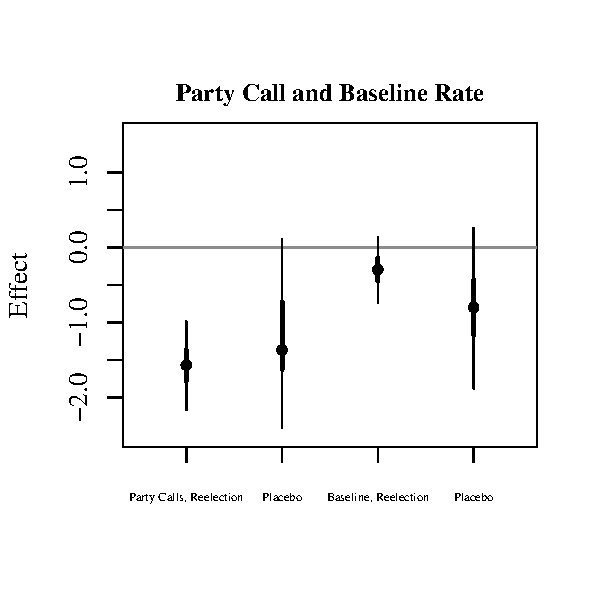
\includegraphics[width = 10cm]{C:/Users/Ethan/Documents/GitHub/partycalls/plots/senate-diff-in-diff-coeff-separate.pdf}
\end{figure}

\begin{figure}[H]
	\centering
	\caption{Senate Rate of Voting With Party by Vote Type}
	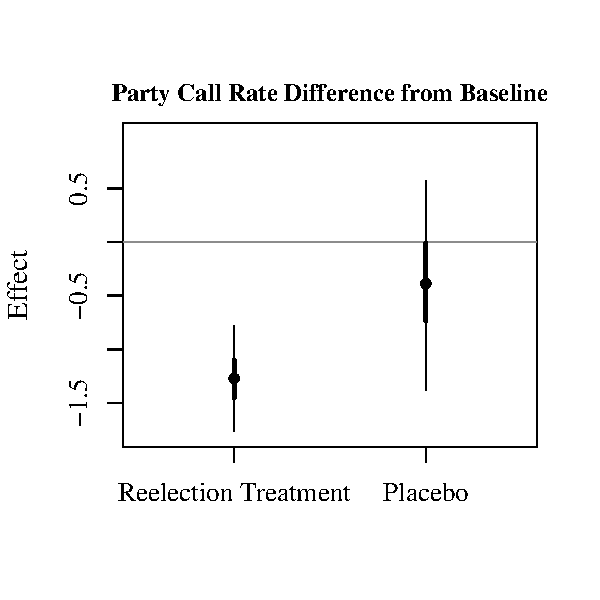
\includegraphics[width = 10cm]{C:/Users/Ethan/Documents/GitHub/partycalls/plots/senate-diff-in-diff-coeff.pdf}
\end{figure}

These show clearly that member responsiveness to party calls declines by approximately 1.5\%. Since the average number of party calls in a Congress during the time we analyze is approximately 365, this means that a Senate party can generally expect to count on members up for reelection for a little over 5 votes against the party on party call votes. Member voting behavior on other votes does not exhibit this relationship. Thus, we are confident in our hypothesis that members respond to the desire of voters

\subsection{Conclusion}

In this paper, we show that members respond to party calls in the Senate as they do in the House using similar analysis to Minozzi \& Volden (2013). Further, in the Senate we are able to consider the role that proximity to reelection has in responsiveness to the party in Congress. Across multiple statistical tests we find that in Congresses which a member is up for reelection there is a lowered responsiveness to the party, demonstrating the way in which members balance the needs of the party with the desires of their constituents given the costs for foregoing either.

\pagebreak

\section{Appendices}

\subsection{Appendix A: Detailing the New Sorting Algorithm}

As in Minozzi \& Volden (2013) we develop an algorithm to sort votes based on the degree to which vote choice can be significantly predicted by party when vote choice is modeled by party and ideology. This algorithm works iteratively, with member ideology in one iteration calculated on the votes which were not party calls in the previous iteration, with the ideology for the first iteration being set as votes which have more than 65\% or less than 35\% of members voting on a bill on the same side. The algorithm must run 15 iterations per Congress as a burn-in period. Once this period has concluded the algorithm continues either until the number of votes switched has hit a minimum and begun to climb or until there are fewer than 5 votes which switch between iterations. Once these conditions are met, it continues for 15 additional iterations, the last 5 of which are used to identify party calls and non calls. Any votes which switched between party calls and non party calls during the final five iterations are dropped from our analyses.

We find that the results produced by the algorithm largely do not involve a tradeoff of party and ideology explaining votes, but instead typically have both explaining effects in the same direction. We have made some changes to this algorithm, which are detailed below.

% latex table generated in R 3.3.2 by xtable 1.8-2 package
% Thu Feb 23 17:39:42 2017
\begin{table}[H]
	\centering
	\caption{House Sorting Algorithm Coefficient Signs}
	\begin{tabular}{rrr}
		\hline
		& ($-$) Ideal & (+) Ideal \\ 
		\hline
		(-) Party & 0.38 & 0.15 \\ 
		(+) Party & 0.17 & 0.30 \\ 
		\hline
	\end{tabular}
\end{table}

% latex table generated in R 3.3.2 by xtable 1.8-2 package
% Thu Feb 23 17:23:31 2017
\begin{table}[H]
	\centering
	\caption{Senate Sorting Algorithm Coefficient Signs}
	\begin{tabular}{rrr}
		\hline
		& ($-$) Ideal & (+) Ideal \\ 
		\hline
		($-$) Party & 0.33 & 0.16 \\ 
		(+) Party & 0.23 & 0.28 \\ 
		\hline
	\end{tabular}
\end{table}

One of the key changes was the use of the \verb|emIRT()| R function as described in Imai, Lo \& Olmsted (2016) in order to obtain members' party free ideology. This function was developed by Imai and co-authors in order to produce estimates analagous to those of the \verb|ideal()| function developed by Clinton, Jackman \& Rivers (2004), which was used by Minozzi \& Volden (2013). A key advantage of this new function for estimation of member ideology is that it produces results with greatly reduced computation.

We found that the lowered number of both members and bills in the Senate required a few changes to the vote sorting method. First, since p-values will necessarily be lower with fewer observations, we had to change the p-value threshold for party significance to 0.05 (from 0.01). Next, since the ideal point algorithm uses a logistic regression problems arose in vote sorting when we also tried to use a logistic regression in the Senate and changed to using a linear model. Neither change leads the sorting in the House to change drastically and we find that the sorting of votes based on whether they are close or lopsided mirrors that found in Minozzi \& Volden (2013) very closely.

% latex table generated in R 3.3.2 by xtable 1.8-2 package
% Mon Mar 20 13:02:44 2017
\begin{table}[H]
	\centering
	\caption{House Vote Coding for Close and Lopsided Votes} 
	\begin{tabular}{lrr}
		\hline
		& Party Call & Noncall \\ 
		\hline
		Lopsided & 4245 & 6123 \\ 
		Close & 9308 & 1090 \\ 
		\hline
	\end{tabular}
\end{table}

% latex table generated in R 3.3.2 by xtable 1.8-2 package
% Mon Mar 20 13:04:18 2017
\begin{table}[H]
	\centering
	\caption{Senate Vote Coding for Close and Lopsided Votes} 
	\begin{tabular}{lrr}
		\hline
		& Party Call & Noncall \\ 
		\hline
		Lopsided & 2063 & 4876 \\ 
		Close & 5233 & 1851 \\ 
		\hline
	\end{tabular}
\end{table}













\subsection{Appendix B: Methodology for Senate Reelection Section}

In order to better test the role of reelection we use same-state senators as a natural pairing. We view this as an ideal pairing since they answer to the same possible set of voters and therefore should have similar preferences induced by proximity to reelection. The tests we performed on these pairs were generalizations of the difference in differences design in which the member not up for reelection had their response rate subtracted from that of the member who was up for reelection for the first figure in the paper and for the second members had the difference between their party call response rate and baseline rate of voting with the party subtracted from that of the other Senator from their state under the same conditions. 

Here we show the effects in tables, along with breakdowns by seat pair type. We additionally show the results of a model with fixed effects by member and Congress. This produces substantively similar effects to those reported in the main paper on the effects of being up for reelection and changes in ideological extremism. This is presented as a robustness check for the results we present in the paper.

% latex table generated in R 3.3.2 by xtable 1.8-2 package
% Mon Mar 27 22:28:47 2017
\begin{table}[H]
	\centering
	\caption{Reelection and Response to Party Calls, Difference in Differences} 
	\begin{tabular}{llrrr}
		\hline
		test & DV & Estimate & Lower\_Bound & Upper\_Bound \\ 
		\hline
		Effect & pirate100 & -1.569 & -2.139 & -1.001 \\ 
		Placebo & pirate100 & -0.331 & -1.281 & 1.259 \\ 
		Effect & pfrate100 & -0.297 & -0.798 & 0.126 \\ 
		Placebo & pfrate100 & -0.644 & -1.074 & 1.143 \\ 
		\hline
	\end{tabular}
\end{table}

% latex table generated in R 3.3.2 by xtable 1.8-2 package
% Mon Mar 27 22:28:47 2017
\begin{table}[H]
	\centering
	\caption{Diff in Diff, Subgroup Condition, Party Influenced Rate} 
	\begin{tabular}{llr}
		\hline
		Test & DV & Estimate \\ 
		\hline
		2 Maj Dems Effect & pirate100 & 0.0708958 \\ 
		2 Maj Dems Placebo & pirate100 & 0.0859113 \\ 
		2 Min Dems Effect & pirate100 & -1.8733904 \\ 
		2 Min Dems Placebo & pirate100 & 0.1595294 \\ 
		2 Maj Reps Effect & pirate100 & -1.1307379 \\ 
		2 Maj Reps Placebo & pirate100 & 0.1677148 \\ 
		2 Min Reps Effect & pirate100 & 0.3990873 \\ 
		2 Min Reps Placebo & pirate100 & -0.1514964 \\ 
		Split, Maj Dem, Dem Effect & pirate100 & 3.8789004 \\ 
		Split, Maj Dem, Dem Placebo & pirate100 & -40.3593458 \\ 
		Split, Maj Dem, Rep Effect & pirate100 & -8.6767819 \\ 
		Split, Maj Dem, Rep Placebo & pirate100 & -42.2647881 \\ 
		Split, Maj Rep, Dem Effect & pirate100 & -8.0169523 \\ 
		Split, Maj Rep, Dem Placebo & pirate100 & -42.4436232 \\ 
		Split, Maj Rep, Rep Effect & pirate100 & 0.0096892 \\ 
		Split, Maj Rep, Rep Placebo & pirate100 & -44.6050484 \\ 
		\hline
	\end{tabular}
\end{table}

% latex table generated in R 3.3.2 by xtable 1.8-2 package
% Sun Mar 26 19:10:24 2017
\begin{table}[H]
	\centering
	\caption{Reelection and Response to Party Calls, Difference in Differences} 
	\begin{tabular}{llrrr}
		\hline
		test & DV & Estimate & Lower\_Bound & Upper\_Bound \\ 
		\hline
		Effect & pirate100 - pfrate100 & -1.272 & -1.775 & -0.794 \\ 
		Placebo & pirate100 - pfrate100 & -0.292 & -0.904 & 0.935 \\ 
		\hline
	\end{tabular}
\end{table}

% latex table generated in R 3.3.2 by xtable 1.8-2 package
% Sun Mar 26 19:10:27 2017
\begin{table}[H]
	\centering
	\caption{Diff in Diff, Subgroup Condition, Party Influenced Rate} 
	\begin{tabular}{llr}
		\hline
		Test & DV & Estimate \\ 
		\hline
		2 Maj Dems Effect & pirate100 - pfrate100 & -0.1191943 \\ 
		2 Maj Dems Placebo & pirate100 - pfrate100 & 0.5657017 \\ 
		2 Min Dems Effect & pirate100 - pfrate100 & -1.8253378 \\ 
		2 Min Dems Placebo & pirate100 - pfrate100 & -0.4463733 \\ 
		2 Maj Reps Effect & pirate100 - pfrate100 & -2.2112471 \\ 
		2 Maj Reps Placebo & pirate100 - pfrate100 & -0.1749949 \\ 
		2 Min Reps Effect & pirate100 - pfrate100 & 0.7774782 \\ 
		2 Min Reps Placebo & pirate100 - pfrate100 & -0.4516436 \\ 
		Split, Maj Dem, Dem Effect & pirate100 - pfrate100 & -0.8756821 \\ 
		Split, Maj Dem, Dem Placebo & pirate100 - pfrate100 & -1.8454871 \\ 
		Split, Maj Dem, Rep Effect & pirate100 - pfrate100 & -1.4582552 \\ 
		Split, Maj Dem, Rep Placebo & pirate100 - pfrate100 & 0.0117995 \\ 
		Split, Maj Rep, Dem Effect & pirate100 - pfrate100 & -7.1166813 \\ 
		Split, Maj Rep, Dem Placebo & pirate100 - pfrate100 & -3.4630959 \\ 
		Split, Maj Rep, Rep Effect & pirate100 - pfrate100 & 0.3772151 \\ 
		Split, Maj Rep, Rep Placebo & pirate100 - pfrate100 & 0.2964502 \\ 
		\hline
	\end{tabular}
\end{table}

\begin{table}[H]
	\begin{center}
		\caption{Senate Fixed Effects Models, Party Call Response Rate}
		\begin{tabular}{l c c c c }
			\hline
			& Democrats & Republicans & Majority & Minority \\
			\hline
			Ideological Extremism  & $2.88^{***}$ & $4.00^{***}$  & $1.80^{**}$   & $3.93^{***}$ \\
			& $(0.69)$     & $(0.75)$      & $(0.64)$      & $(0.97)$     \\
			Baseline Rate of Voting with Party               & $0.37^{***}$ & $0.25^{***}$  & $0.37^{***}$  & $0.18^{*}$   \\
			& $(0.05)$     & $(0.05)$      & $(0.05)$      & $(0.07)$     \\
			Up For Reelection     & $-0.55^{*}$  & $-1.55^{***}$ & $-1.02^{***}$ & $-1.04^{**}$ \\
			& $(0.27)$     & $(0.34)$      & $(0.28)$      & $(0.37)$     \\
			Vote Share             & $0.03$       & $-0.05$       & $0.02$        & $-0.02$      \\
			& $(0.02)$     & $(0.03)$      & $(0.03)$      & $(0.04)$     \\
			Presidential Vote Share       & $0.27^{***}$ & $0.09$        & $0.31^{***}$  & $0.14^{*}$   \\
			& $(0.04)$     & $(0.05)$      & $(0.06)$      & $(0.06)$     \\
			Freshman                & $0.71$       & $0.98^{*}$    & $0.77$        & $0.78$       \\
			& $(0.48)$     & $(0.46)$      & $(0.46)$      & $(0.76)$     \\
			Retiree                 & $0.25$       & $0.88$        & $0.36$        & $0.75$       \\
			& $(0.83)$     & $(0.83)$      & $(0.99)$      & $(0.91)$     \\
			Best Committee         & $0.14$       & $0.11$        & $0.29$        & $0.36^{*}$   \\
			& $(0.12)$     & $(0.16)$      & $(0.15)$      & $(0.18)$     \\
			Power Committee        & $-0.48$      & $-0.22$       & $-1.26$       & $-0.45$      \\
			& $(0.70)$     & $(0.98)$      & $(0.89)$      & $(1.01)$     \\
			Leader                  & $0.87$       & $1.46^{*}$    & $1.39$        & $1.31$       \\
			& $(0.47)$     & $(0.62)$      & $(0.78)$      & $(0.80)$     \\
			Committee Chair                   & $0.38$       & $0.65$        & $-0.57$       &              \\
			& $(0.64)$     & $(0.71)$      & $(0.56)$      &              \\
			\hline
			Num. obs.               & 1042         & 951           & 1052          & 843          \\
			R$^2$      & 0.89         & 0.91          & 0.92          & 0.94         \\
			Adj. R$^2$ & 0.87         & 0.88          & 0.89          & 0.91         \\
			\hline
			\multicolumn{5}{l}{\scriptsize{$^{***}p<0.001$, $^{**}p<0.01$, $^*p<0.05$}}
		\end{tabular}
	\end{center}
\end{table}

\subsection{Appendix C: Other Tables and Figures from Replication}
\begin{table}
	\begin{center}
		\caption{Statistical models}
		\begin{tabular}{l c c c c c c }
			\hline
			& \multicolumn{3}{c}{Democrats} & \multicolumn{3}{c}{Republicans} \\
			\cline{2-7}
			& 97th & 102nd & 107th & 97th & 102nd & 107th \\
			\hline
			ideological\_extremism & $9.27^{***}$  & $5.07^{***}$  & $-1.11$      & $5.21^{***}$ & $6.78^{***}$  & $-0.20$       \\
			& $(0.53)$      & $(0.69)$      & $(1.50)$     & $(0.71)$     & $(0.76)$      & $(0.61)$      \\
			pfrate100              & $1.03^{***}$  & $0.67^{***}$  & $1.11^{**}$  & $0.50^{***}$ & $0.48^{***}$  & $0.35^{**}$   \\
			& $(0.07)$      & $(0.08)$      & $(0.36)$     & $(0.08)$     & $(0.08)$      & $(0.11)$      \\
			pres\_votepct          & $0.15^{**}$   & $0.14^{**}$   & $0.22^{***}$ & $0.23^{***}$ & $0.21^{*}$    & $0.18^{***}$  \\
			& $(0.05)$      & $(0.05)$      & $(0.06)$     & $(0.07)$     & $(0.08)$      & $(0.03)$      \\
			south                  & $-4.20^{***}$ & $-1.31$       & $-3.13^{*}$  & $1.53$       & $0.07$        & $1.75^{***}$  \\
			& $(1.02)$      & $(0.80)$      & $(1.28)$     & $(1.19)$     & $(1.22)$      & $(0.52)$      \\
			votepct                & $-0.08^{*}$   & $-0.03$       & $-0.04$      & $0.05$       & $-0.00$       & $-0.03$       \\
			& $(0.03)$      & $(0.03)$      & $(0.05)$     & $(0.05)$     & $(0.03)$      & $(0.02)$      \\
			female                 & $0.05$        & $-1.58$       & $2.44^{*}$   & $-4.21^{*}$  & $-1.87$       & $-1.39$       \\
			& $(2.06)$      & $(1.22)$      & $(1.21)$     & $(2.00)$     & $(2.25)$      & $(0.83)$      \\
			afam                   & $-2.56$       & $-1.98$       & $-1.43$      &              & $3.95$        & $-3.54$       \\
			& $(2.12)$      & $(1.58)$      & $(1.73)$     &              & $(6.14)$      & $(3.57)$      \\
			latino                 & $4.02$        & $2.79$        & $0.69$       & $-1.28$      & $3.26$        & $0.79$        \\
			& $(2.91)$      & $(1.90)$      & $(1.89)$     & $(5.75)$     & $(6.35)$      & $(1.50)$      \\
			seniority              & $0.08$        & $0.07$        & $-0.11$      & $-0.02$      & $-0.71^{***}$ & $-0.17^{*}$   \\
			& $(0.12)$      & $(0.10)$      & $(0.13)$     & $(0.17)$     & $(0.15)$      & $(0.08)$      \\
			freshman               & $-1.25$       & $0.01$        & $-0.13$      & $3.45^{*}$   & $3.76^{*}$    & $0.59$        \\
			& $(1.43)$      & $(1.19)$      & $(2.02)$     & $(1.34)$     & $(1.77)$      & $(0.78)$      \\
			bestgrosswart          & $0.09$        & $-0.06$       & $0.25^{*}$   & $0.11$       & $0.11$        & $0.17^{**}$   \\
			& $(0.08)$      & $(0.08)$      & $(0.10)$     & $(0.09)$     & $(0.11)$      & $(0.05)$      \\
			leader                 & $7.02^{*}$    & $2.00$        & $0.56$       & $0.38$       & $4.26$        & $3.17^{*}$    \\
			& $(2.87)$      & $(1.95)$      & $(2.42)$     & $(2.42)$     & $(2.24)$      & $(1.23)$      \\
			power                  & $1.09$        & $1.44$        & $-1.23$      & $-1.37$      & $-0.03$       & $-0.21$       \\
			& $(1.02)$      & $(0.90)$      & $(1.31)$     & $(1.35)$     & $(1.41)$      & $(0.63)$      \\
			chair                  & $2.61$        & $1.31$        &              &              &               & $1.30$        \\
			& $(1.52)$      & $(1.35)$      &              &              &               & $(0.91)$      \\
			(Intercept)            & $-18.03^{**}$ & $25.29^{***}$ & $-33.70$     & $11.17$      & $23.11^{**}$  & $47.81^{***}$ \\
			& $(6.71)$      & $(7.32)$      & $(35.43)$    & $(8.06)$     & $(8.49)$      & $(10.27)$     \\
			\hline
			R$^2$                  & 0.82          & 0.65          & 0.36         & 0.54         & 0.61          & 0.52          \\
			Adj. R$^2$             & 0.80          & 0.64          & 0.31         & 0.50         & 0.58          & 0.49          \\
			Num. obs.              & 233           & 263           & 209          & 187          & 162           & 217           \\
			RMSE                   & 5.47          & 4.97          & 6.39         & 5.62         & 5.86          & 3.26          \\
			\hline
			\multicolumn{7}{l}{\scriptsize{$^{***}p<0.001$, $^{**}p<0.01$, $^*p<0.05$}}
		\end{tabular}
	\end{center}
\end{table}

\begin{figure}[H]
	\centering
	\caption{House Ideological Extremism Coefficient Plot}
	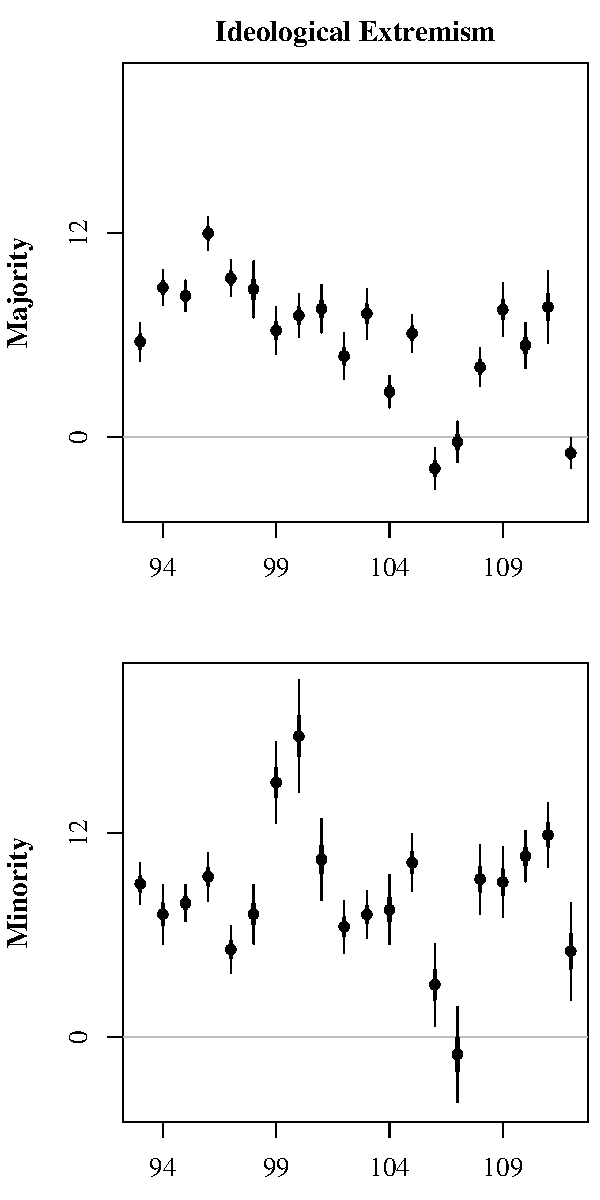
\includegraphics[width = 10cm]{C:/Users/Ethan/Documents/GitHub/partycalls/plots/who-heeds-figure2-replication_lm.pdf}
\end{figure}

\begin{figure}[H]
	\centering
	\caption{Senate Ideological Extremism Coefficient Plot}
	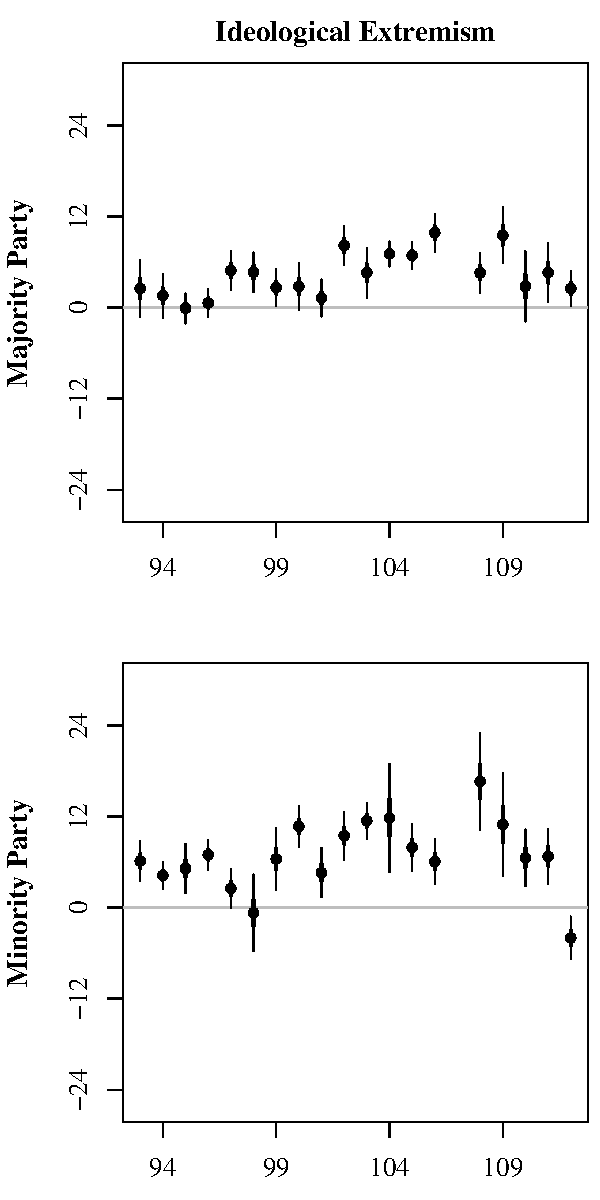
\includegraphics[width = 10cm]{C:/Users/Ethan/Documents/GitHub/partycalls/plots/senate-figure2-lm.pdf}
\end{figure}





















































\end{document}